\section{Tools} \label{sec:tools}

This section of the paper describes the tools used for the scrub process. With the requirement for agility, collaborative working and ease of linking to existing tools, google suite is the chosen platform onto which the scrub tools have been developed. The tool, called the Scrub Sandbox,  need to facilitate the following:

\begin{enumerate}
\item Capturing the current state.
\item Capturing what the the desired change is.
\item Inputting flow down milestones for the upcoming FY based on higher level milestones defined by the Director’s office
\item Standardized inputs
\item Easily seeing the impact of the desired change on labor and non-labor budget.
\end{enumerate}

\begin{figure}
\begin{centering}
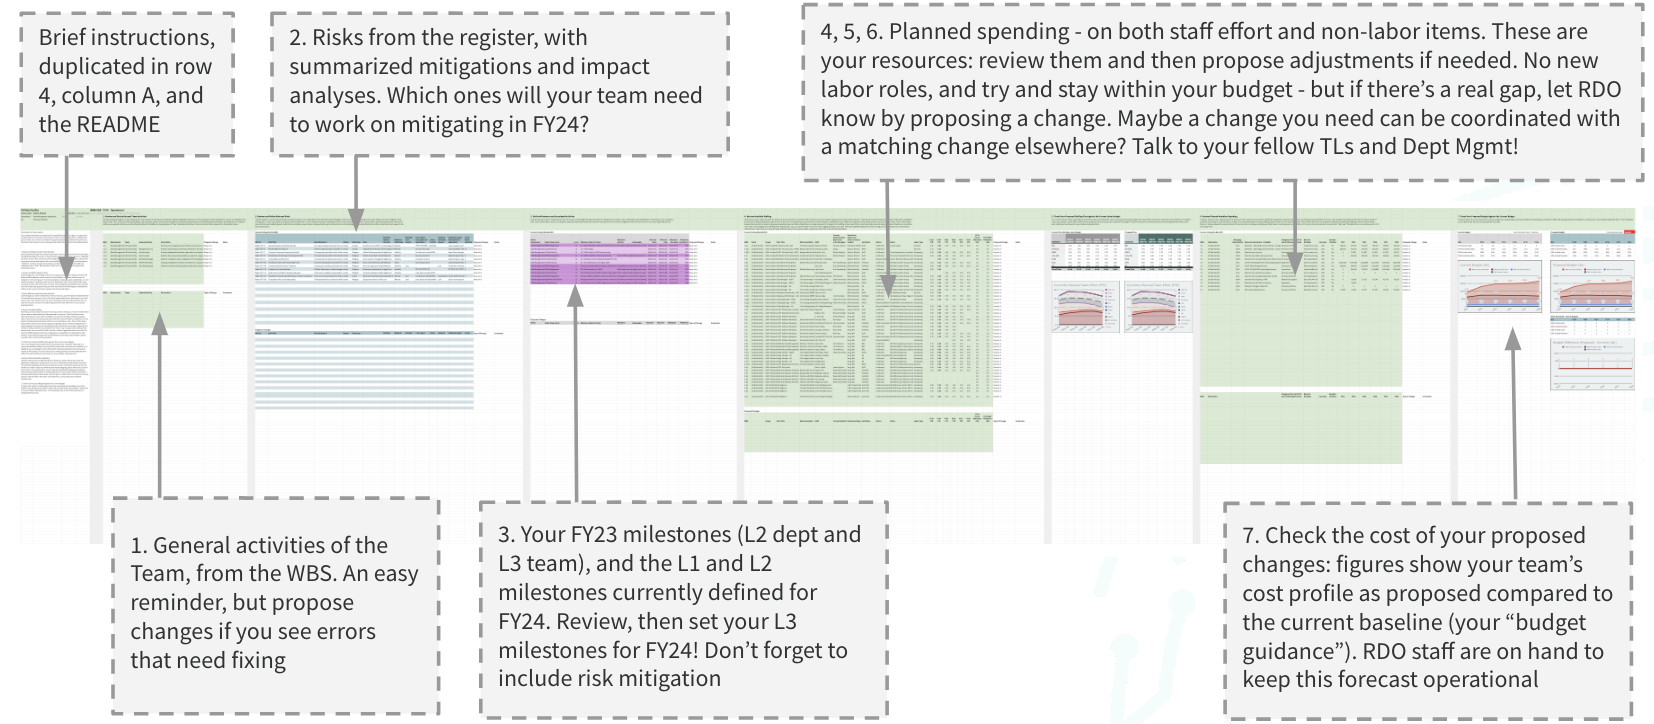
\includegraphics[\textwidth]{Figure3OverviewScrubSandbox}
	\caption{ Overview of Scrub Sandbox
\label{fig:sandbox}}
\end{centering}
\end{figure}


Furthermore, the tool needs to enable the following areas to be scrubbed:
\begin{enumerate}
\item Work Breakdown Structure (WBS)
\item Risks.
\item Milestones.
\item Labor expenditure.
\item Non-labor expenditure.
\end{enumerate}

In all the above cases a standard approach is applied to propose changes See \autoref{fig:wbs}. Beside the current activity in the Proposed Change column during the scrub review a value is chosen from the drop down choices which are Keep As-Is, Modify, Remove/Replace. There is space to enter a note if explanation is needed.
A Modify proposal will require a corresponding entry in the Proposed Changes table directly below the current status table as will proposed Additions.
Proposed changes to the labor and non-labor plan are visualized in monetary terms in real-time with baseline comparison charts such as those shown in \autoref{fig:baseline}.



\begin{figure}
\begin{centering}
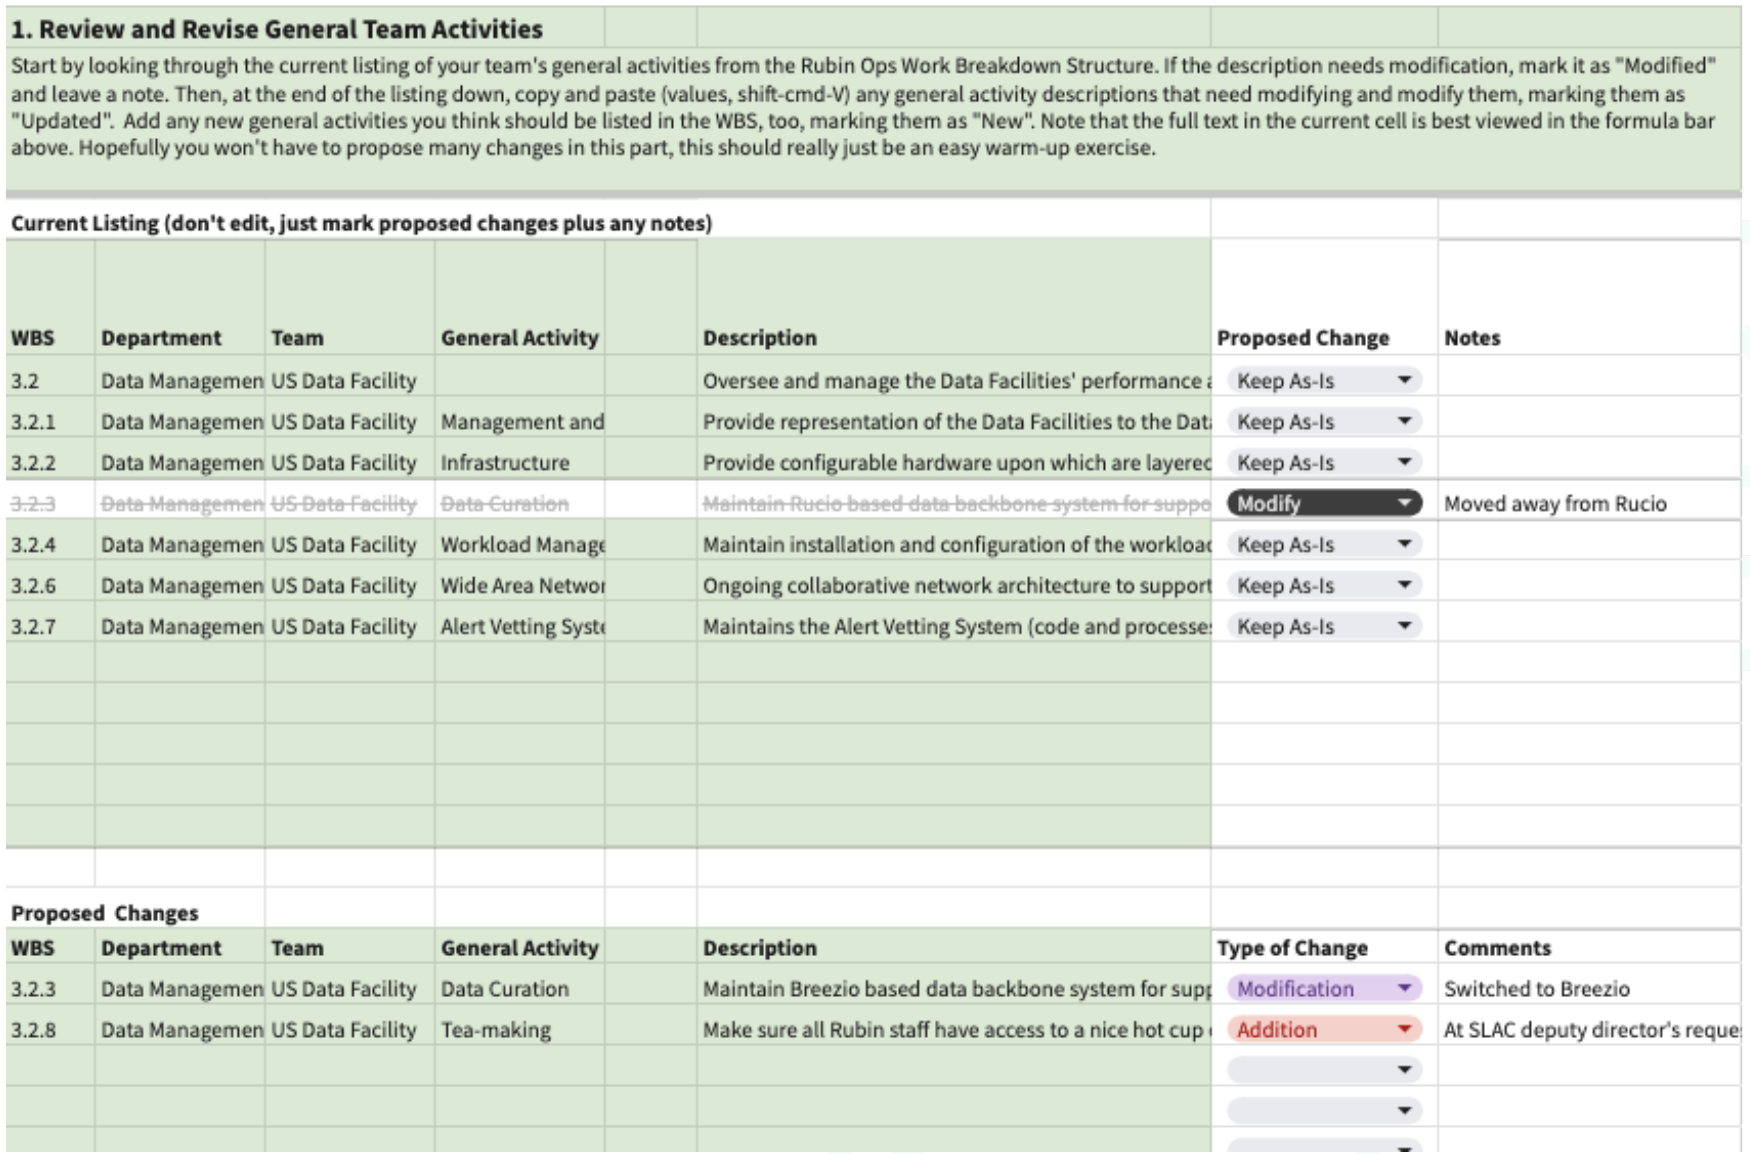
\includegraphics[\textwidth]{Figure4WorkBreakdownStructurescrubbing}
	\caption{ Work Breakdown Structure scrubbing
\label{fig:wbs}}
\end{centering}
\end{figure}

\begin{figure}
\begin{centering}
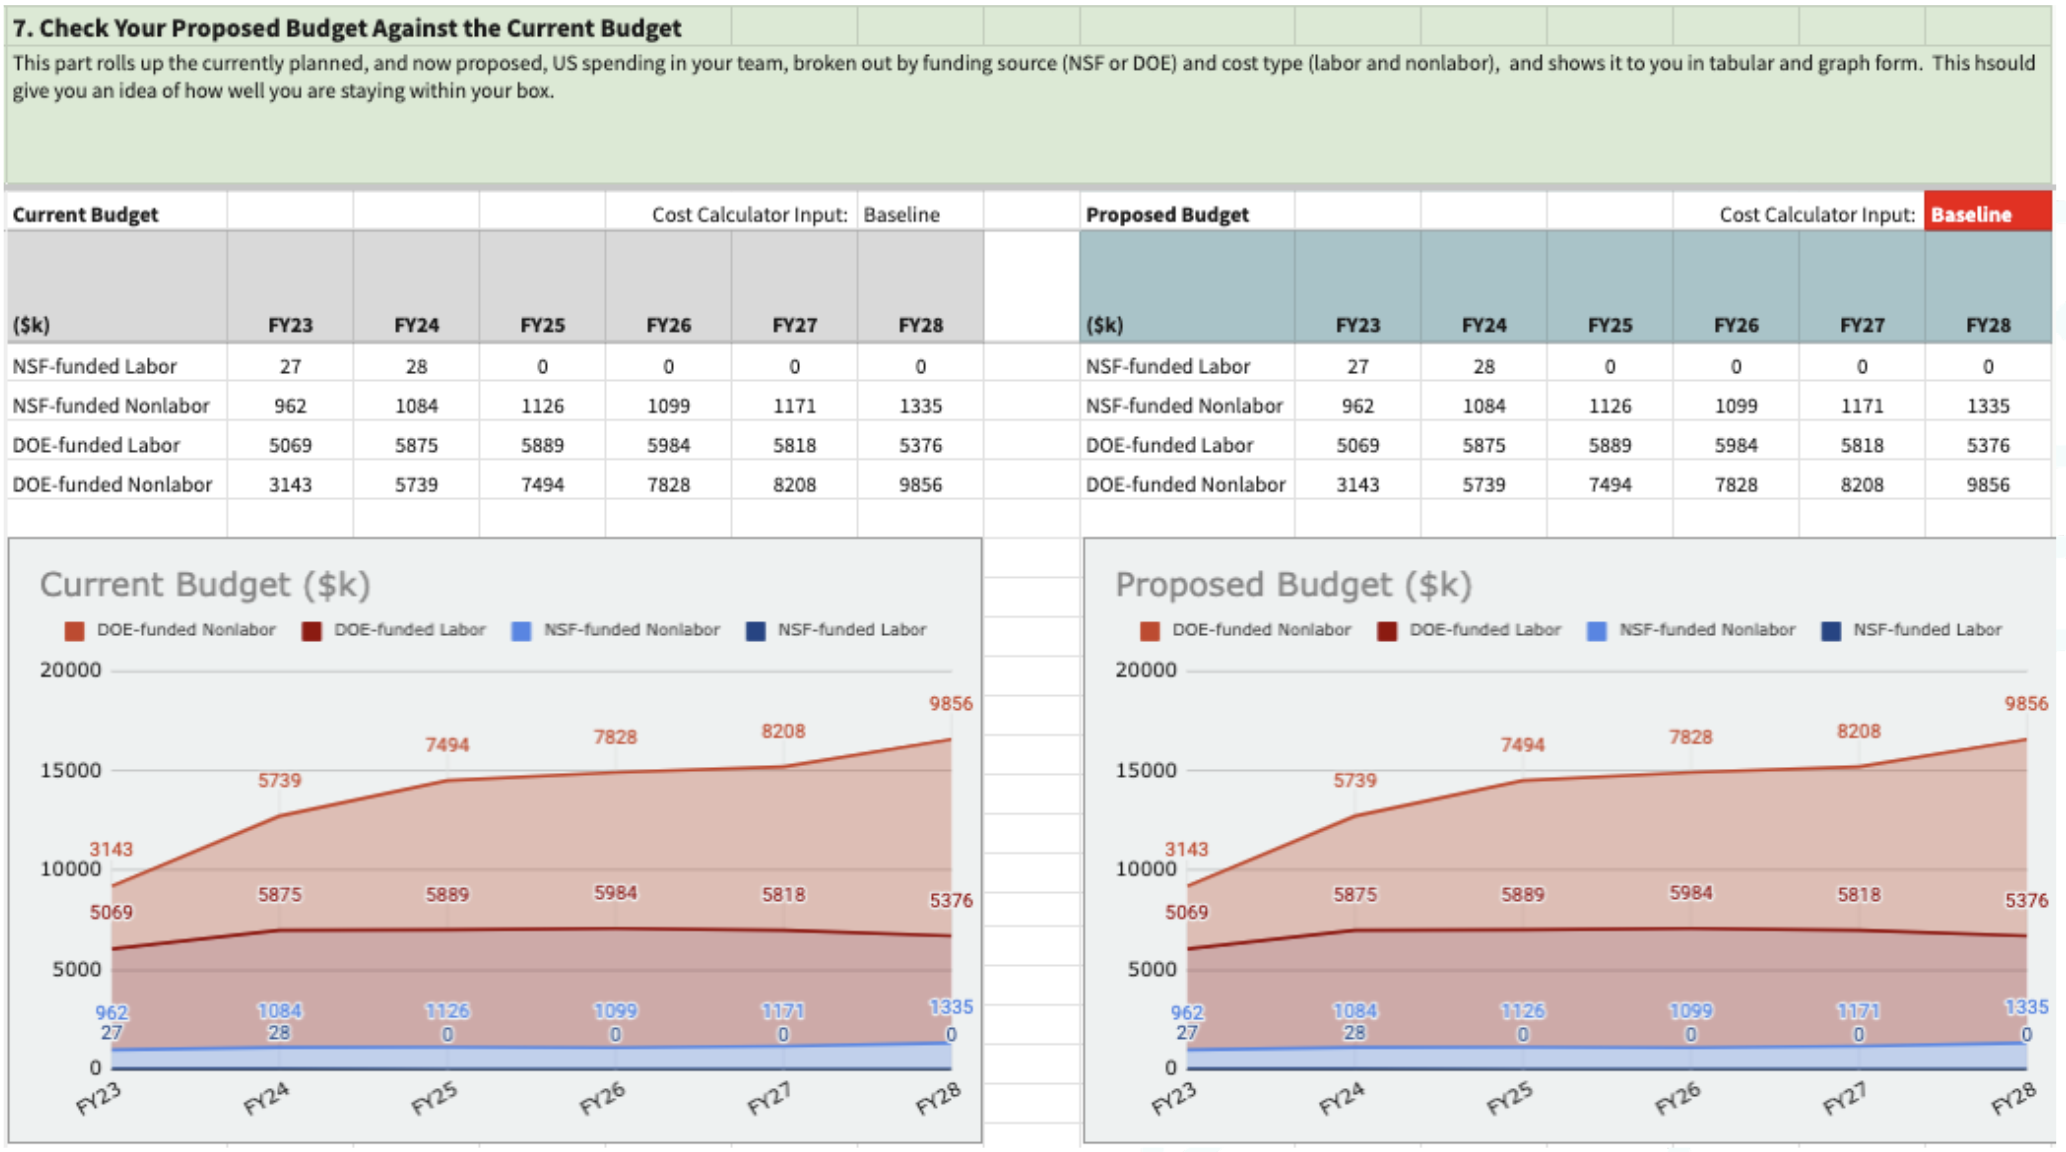
\includegraphics[\textwidth]{Figure5BaselinevsProposed}
	\caption{Baseline vs Proposed labor and non-labor comparison
\label{fig:baseline}}
\end{centering}
\end{figure}
